\documentclass[11pt]{article}

\usepackage[letterpaper,top=1.8cm,bottom=2cm,left=2.5cm,right=2.5cm,marginparwidth=1.75cm]{geometry}

%packages
\usepackage{amsmath}
\usepackage{graphicx}
\usepackage{amssymb}
\usepackage{algorithm}
\usepackage{algpseudocode}
\usepackage{color,soul}
\usepackage{mathtools}
% \usepackage{subfig}
\usepackage{subcaption}
\usepackage{caption}

% Edits by John:
% Use hyperref when you're referencing anything - in particular, use the \autoref{} command - it's great. One exception: anything in mathmode should be referenced using \eqref{} instead; \autoref{} calls all mathmode objects "equations", even when they're not equations (definitions, inequalities, propositions, statements, etc.), so it's better to use the \eqref{} function.
\usepackage[colorlinks, linkcolor=blue, citecolor=blue, urlcolor=blue]{hyperref}
\newcommand{\algorithmautorefname}{Algorithm}
% Use the align (or similar) environment, rather than built-in latex commands for math statements. That way, things can be aligned properly and equations will be numbered and referencable. The equation below assigns equation numbers based upon the current section.

\numberwithin{equation}{section}
% Use the amsthm environents to define theorems, remarks, definitions, etc., with commands of the form \begin{definition}[DEFINITION ITTLE]
\usepackage{amsthm}% provides the environments
\theoremstyle{definition}% provides a style for definitions - this affects all downstream \newtheorem statements until \theoremstyle is used again.
\newtheorem{definition}{Definition}[section]% numbers definitions within sections
% The singular of "matrices" is "matrix", not "matrice" - the abnormal singular-plural pair is an importation from Latin.
% Use \url{} for hyperlinks (I changed the pytorch link). I think this is included in hyperref, but it may be in base LaTeX.

\DeclarePairedDelimiter\ceil{\lceil}{\rceil}
\DeclarePairedDelimiter\floor{\lfloor}{\rfloor}
\newcommand{\pluseq}{\mathrel{+}=}
\newcommand{\asteq}{\mathrel{*}=}

\usepackage[dvipsnames]{xcolor}

\definecolor{lavender}{RGB}{214, 111, 208}
\colorlet{lavender}{lavender!50}

\newcommand{\hlinfo}[1]{{\sethlcolor{lavender}\hl{#1}}}
\newcommand{\note}[1]{\textcolor{red}{[#1]}}

\setlength\parindent{0pt}

\begin{document}

\noindent
\begin{center}
    \section*{\centering{Week 1 Notes}}
    \subsection*{\centering{\emph{Lectures 1 \& 2}}}
    \emph{University of Massachusetts Amherst}, CS389
\end{center}

\section{Supervised Learning (lecture 1)}
\begin{definition}[Machine Learning]
    A program, $p$, is able to perform a task, $t$, better according to some metric, $m$, when given experience, $e$. (Mitchell, 1997)
\end{definition}
\begin{definition}[Model]
A \emph{model} is some structure that uses parameters to define a function. An example of a model is $y= wx + b$, which is a linear model. In another more explicit notation, we might write a linear model as (refer to \autoref{section:linearconvention} for more info):
\begin{align}
    \hat{y} = \sum_{j=1}^{m}{w_j \cdot X_j + b} = XW^{T} + b,
\end{align}
where we have a weight $w_j$ for each feature $X_j$, a bias term $b$, and an output vector $\hat{y}$. 
\end{definition}

The intuition is that, the parameters (i.e. $W$ and $b$) can be changed based off the data so that the model performs the optimal function/prediction/output. We say that the model learns because it is able learn the right combination of $W$ and $b$ to give an optimal output (global optimality is not guaranteed; we will talk more about this in the next lecture). The weights, $w_j$, determines how important a feature $x_j$ is to the $\hat{y}$. When the parameters of a machine learning model are fixed, the model can be viewed as a function, $F$, of input features $X$:
\begin{align}
    \hat{y} = F(X_1, ..., X_m) = w_1 X_1 + ... + w_m X_m + b.
\end{align}
For example, the inputs of a weather model can be the humidity, temperature, air speed, etc., and the output could be \emph{how much} it will rain (a type of model known as a \emph{regression model}) or a probability distribution of \emph{what} the weather will be like (a type of model known as a \emph{classification model}). In a regression model the output $y \in \mathbb{R}$ while the output of a classification model is a probability distribution $Y \sim p(x)$. A classification model with 2 classes is a binary classification model, and a model with 2 or more classes is a multi-class classification model.

\begin{definition}[Supervised Learning]
A \emph{supervised learning} system is a system in which we can train a model with labeled data. For example, given an image $x_{1}$ the label $y_{1}$ could be ``dog''. A collection of these is a \emph{dataset}, $D$:
% https://www.cs.cornell.edu/courses/cs4780/2018fa/lectures/lecturenote01_MLsetup.html
\begin{align}
D= \left\{(x_1, y_1), ..., (x_n, y_n)\right\},
\end{align}
where $x_i$ is the input vector to the $i^{\text{th}}$ sample and $y_i$ is the corresponding label to the $i^{\text{th}}$ sample. The goal in supervised learning is to learn a function $F$ such that for a new pair of data $(x, y)$, we have $F(x) \approx y$ with high probability \cite{Cornell}.
\end{definition}

\subsection{Why $\hat{y} = XW^{T} + b$?}
\label{section:linearconvention}
Naively, we can implement a linear model using \autoref{alg:linear_model}. 
\begin{algorithm}
    \caption{Naive Linear Model}
    \begin{algorithmic}[1]
        \State{$y=b$}
        \For{$j$ in range($m$)}
            \State{$y \pluseq w_j \ast x_j$} \Comment{scalar multiplication}
        \EndFor
    \end{algorithmic}
    \label{alg:linear_model}
\end{algorithm}
However, this is a very ugly implementation and for-loops in Python are slow. For our implementation, it would be better to express the operation using matrices. Generally we want $X$ to have shape $(n \times m)$ where $n$ is the number of data and $m$ is the number of features (i.e each row/data has $m$ features), therefore a $(m \times n)$ shape would not make sense. We also want the output to have shape $(n \times p)$ where $p$ are the predictions (i.e. each row/data has $p$ predictions). The problem with $W^TX$ is that we need to transpose the $X$ matrix which does not make sense to do so:
\begin{align}
    (?, ?) \times (n, m) \rightarrow (n, p).
\end{align}
Instead, writing it as $XW^T$ makes more sense:
\begin{align}
    (n,m) \times (?,?) \rightarrow (n,p),
\end{align}
where the weight matrix can now have shape $(m,p)$. However, we want to represent the weight matrix as shape $(p,m)$ as it is equivalent to saying ``a prediction $p$ can be made if given $m$ features''. Therefore, the dimensions of $X$, $W$, and output will be:

\begin{itemize}
    \item {$W \rightarrow (p,m)$}
    \item {$X \rightarrow (n,m)$}
    \item {Out $\rightarrow (n,p)$}
\end{itemize}

We can see this convention being adopted by Pytroch (torch.nn.Linear)\footnote{\url{https://pytorch.org/docs/master/generated/torch.nn.Linear.html}}. Another reason to represent $W$ and $X$ as matrices is that this form is easier to differentiate for gradient descent.

\section{Regression (lecture 1)}
\begin{definition}[Linear Regression]

If we have a linear model (i.e. $y=XW^T+b$) finding the particular parameters ($W$ and $b$) for this linear function is called \emph{linear regression}. You may recall procedures for finding the line of best fit from a previous course - this is the same process, in an arbitrary dimension.
\end{definition}

\section{Loss Function (lecture 2)}
% John: In this section, I adjusted the parentheticals for MAE and MSE; you're using those as mathematical symbols,  and in your mathematics, they are (as they should be) upright. As a result, you should avoid accidentally italicizing them.
% Relatedly, if I were you I would implement the following scheme:
% \newcommand{\MAE}{\text{MAE}}
% \newcommand{\MSE}{\text{MSE}}
% Schemes like this help you to remain consistent in your notation, and make it easier to modify if needed.
\begin{definition}[Loss Function]
A \emph{loss function} measures how \emph{poorly} the model is performing. The lower the loss, the better. A loss of zero means it makes perfect predictions. An example of a well-known loss function is the \emph{Mean Absolute Error} (MAE) and can be written formally as:
\begin{align}
    \text{MAE($y, \hat{y}'$)} = \frac{1}{N}\sum_{n}^{N}{y_n - \hat{y}_n'},
\end{align}
where $y_n$ is the $n^{\text{th}}$ label in the data and $\hat{y}_n'$ is the output of the model when given the $n^{\text{th}}$ data, $x_n$. Another loss function is the \emph{Mean Square Error} (MSE) and can be written formally as:
\begin{align}
    \text{MSE($y, \hat{y}'$)} = \frac{1}{N}\sum_{n}^{N}{(y_n - \hat{y}_n')^2}.
\end{align}
The MAE will prefer outliers while MSE will prefer none to be extremely far. It is common practice to normalize the loss by the total number of training samples, $N$, so that the output can be interpreted as the average loss per sample \cite{Cornell}.

\end{definition}
% \footnote{https://www.cs.cornell.edu/courses/cs4780/2018fa/lectures/lecturenote01_MLsetup.html}. 

\subsection{Properties of the Loss Function}

\begin{enumerate}
    \item {The minimal loss value should correspond to the line of best fit}
    \item {The loss must be defined for all outputs and labels (no divide by 0)}
    \item {The loss function should be differentiable (for gradient descent)}
\end{enumerate}

Therefore, an ideal loss function, $L(w)$, is convex, continuous, and differentiable.

\section{Gradient Descent (lecture 2)}

% John: You should pick either $L$ or Loss for your loss function notation (I would prefer $L$). Using both has the potential to be very confusing. If you're unsure of which to use, converting it to a macro such as
% \newcommand{\Loss}{L}
% would enable you write your mathematics more fluidly.

In the previous section, we described two common loss functions that describes how poor the model is performing. Our goal is to find the optimal set of parameters that minimizes the loss:
\begin{align}% use \arg and \min - two reasons: 1) they are standard, and 2) they are ``math operators''; this affects the way that other commands interact with them. If you ever want something to interact this way (e.g. have super and subscripts go above and below rather than to the right), use \mathop{\symbol}
    W^{\ast} = \arg \min_{W} L(W)
\end{align}% John: Gradient descent is an algorithm independent of computer science and is not synonymous with batch gradient descent. I've adjusted the wording here accordingly.
Clearly, this is an optimization task. The most common tool for finding the optimum in a problem such as this is known as \emph{gradient descent}. There are other ways of performing optimization (i.e. LBFGS) but gradient descent is the most common and established way of optimizing Neural Network loss functions \cite{Stanford}.

\begin{definition}[Gradient of Loss]
    The \emph{gradient of loss}, $\nabla$Loss, is the \emph{direction of steepest ascent}. The negative gradient of loss, $-\nabla$Loss, is the direction of steepest descent. The gradient of loss with respect to the weight can be written as:
    \begin{align}
        \nabla_W \text{Loss} = \frac{\partial L}{\partial W} = \left( \frac{\partial L}{\partial W_1}, \frac{\partial L}{\partial W_2}, ..., \frac{\partial L}{\partial W_m} \right)
    \end{align}
\end{definition}

\begin{definition}[Gradient Descent]
    Is an optimization algorithm that minimizes the loss $L(W)$. The intuition behind the \emph{gradient descent} algorithm is to iteratively update $W_i$ in the direction of the negative gradient (steepest descent) until we converge to the value $W_i$ that is minimized by $L(W_i)$, which can be denoted as $W_i^{\ast}$.  Taking a small enough step, $\alpha$, in the negative gradient is guranteed to reduce loss and convergence to an optimal model. The step size, $\alpha$, is also known as the \emph{learning rate} is a hyperparameter. Formally, we can write all of this as\footnote{Assume that this model has no bias (i.e. $b=0$) for simplicity}:
    \begin{align}
        W = W - \alpha \nabla_W \text{Loss}  
    \end{align}
    \begin{align}
        W_i = W_i - \alpha \frac{\partial L}{\partial W_i}  
    \end{align}
\end{definition}

Whether we converge to an optimal solution depends on how we set the learning rate $\alpha$. The model is unable to converge if $\alpha$ is too large, and is unable/expensive to converge because $\alpha$ is too small. This is visualized in \autoref{fig:learningrate_example}. Usually $\alpha > 0$ and is some small number. We say the model converges when we see that $\frac{\partial L}{\partial w}$ is minimized ($=0)$ or does not change after each iteration of the gradient descent algorithm.

\begin{figure}[h]%
    \centering
    \subfloat[\centering $\alpha$ is just right]{{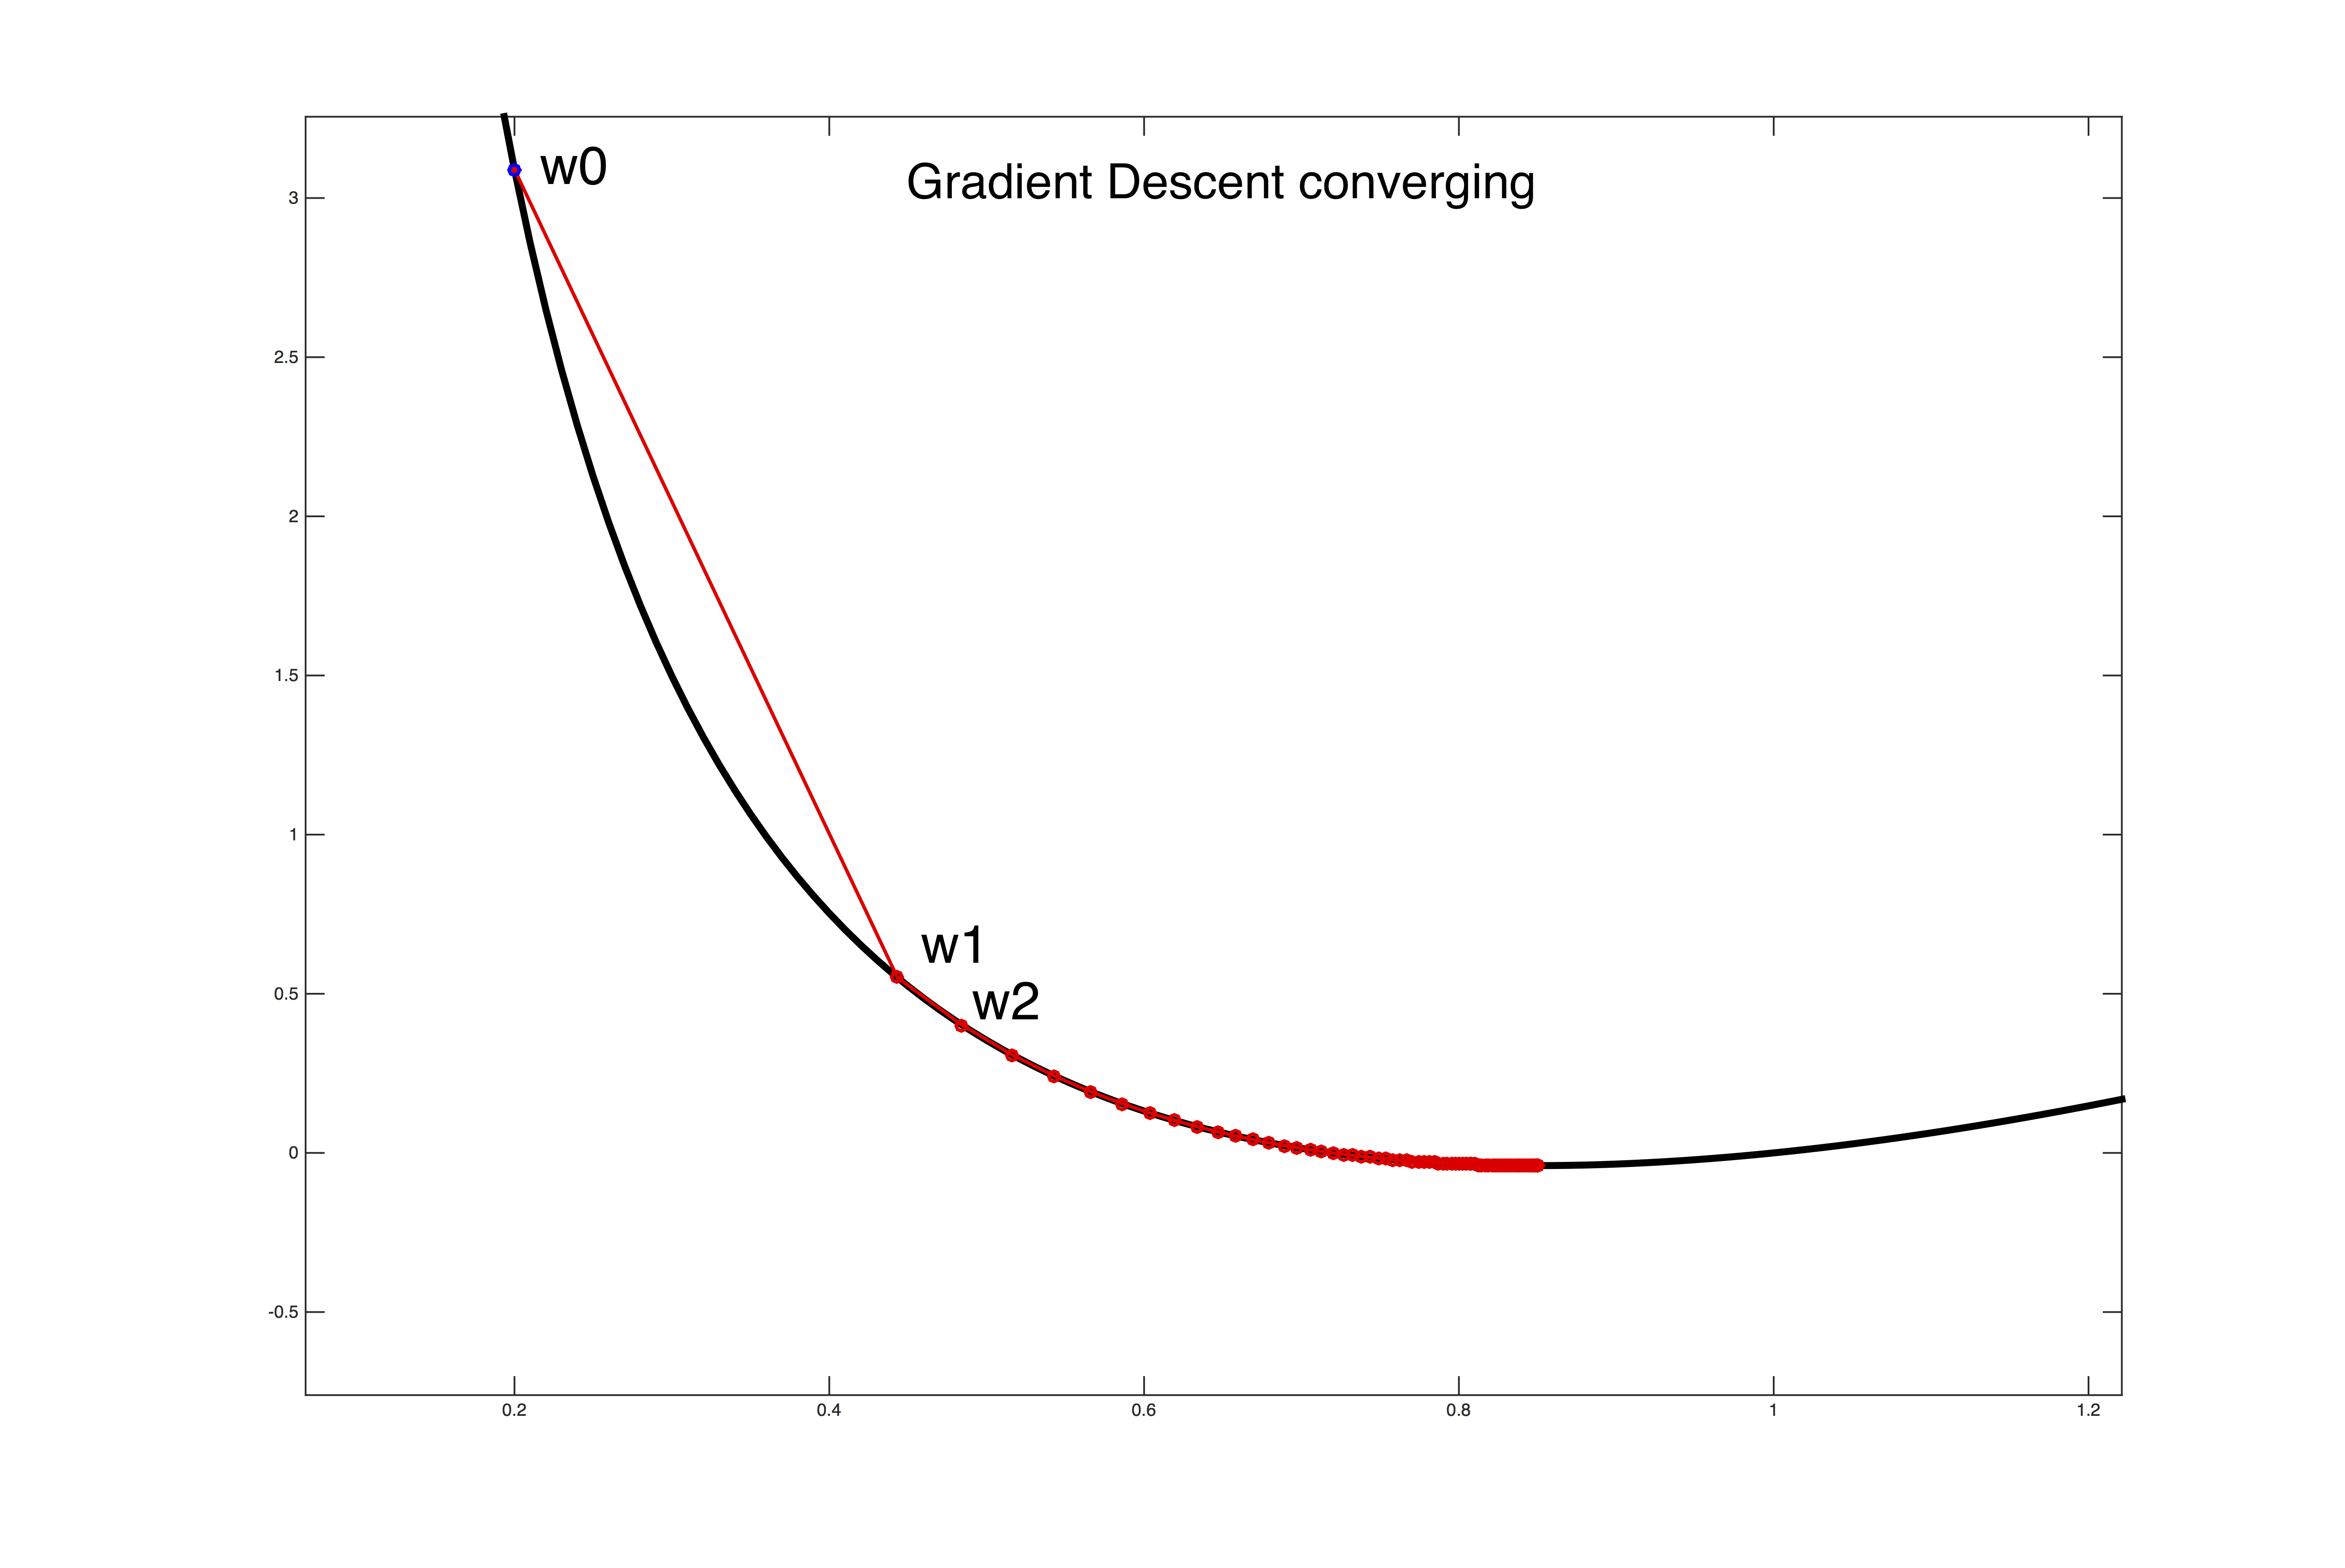
\includegraphics[width=8cm]{./Figs/lr_converge.jpg} }}%
    \qquad
    \subfloat[\centering $\alpha$ is too large]{{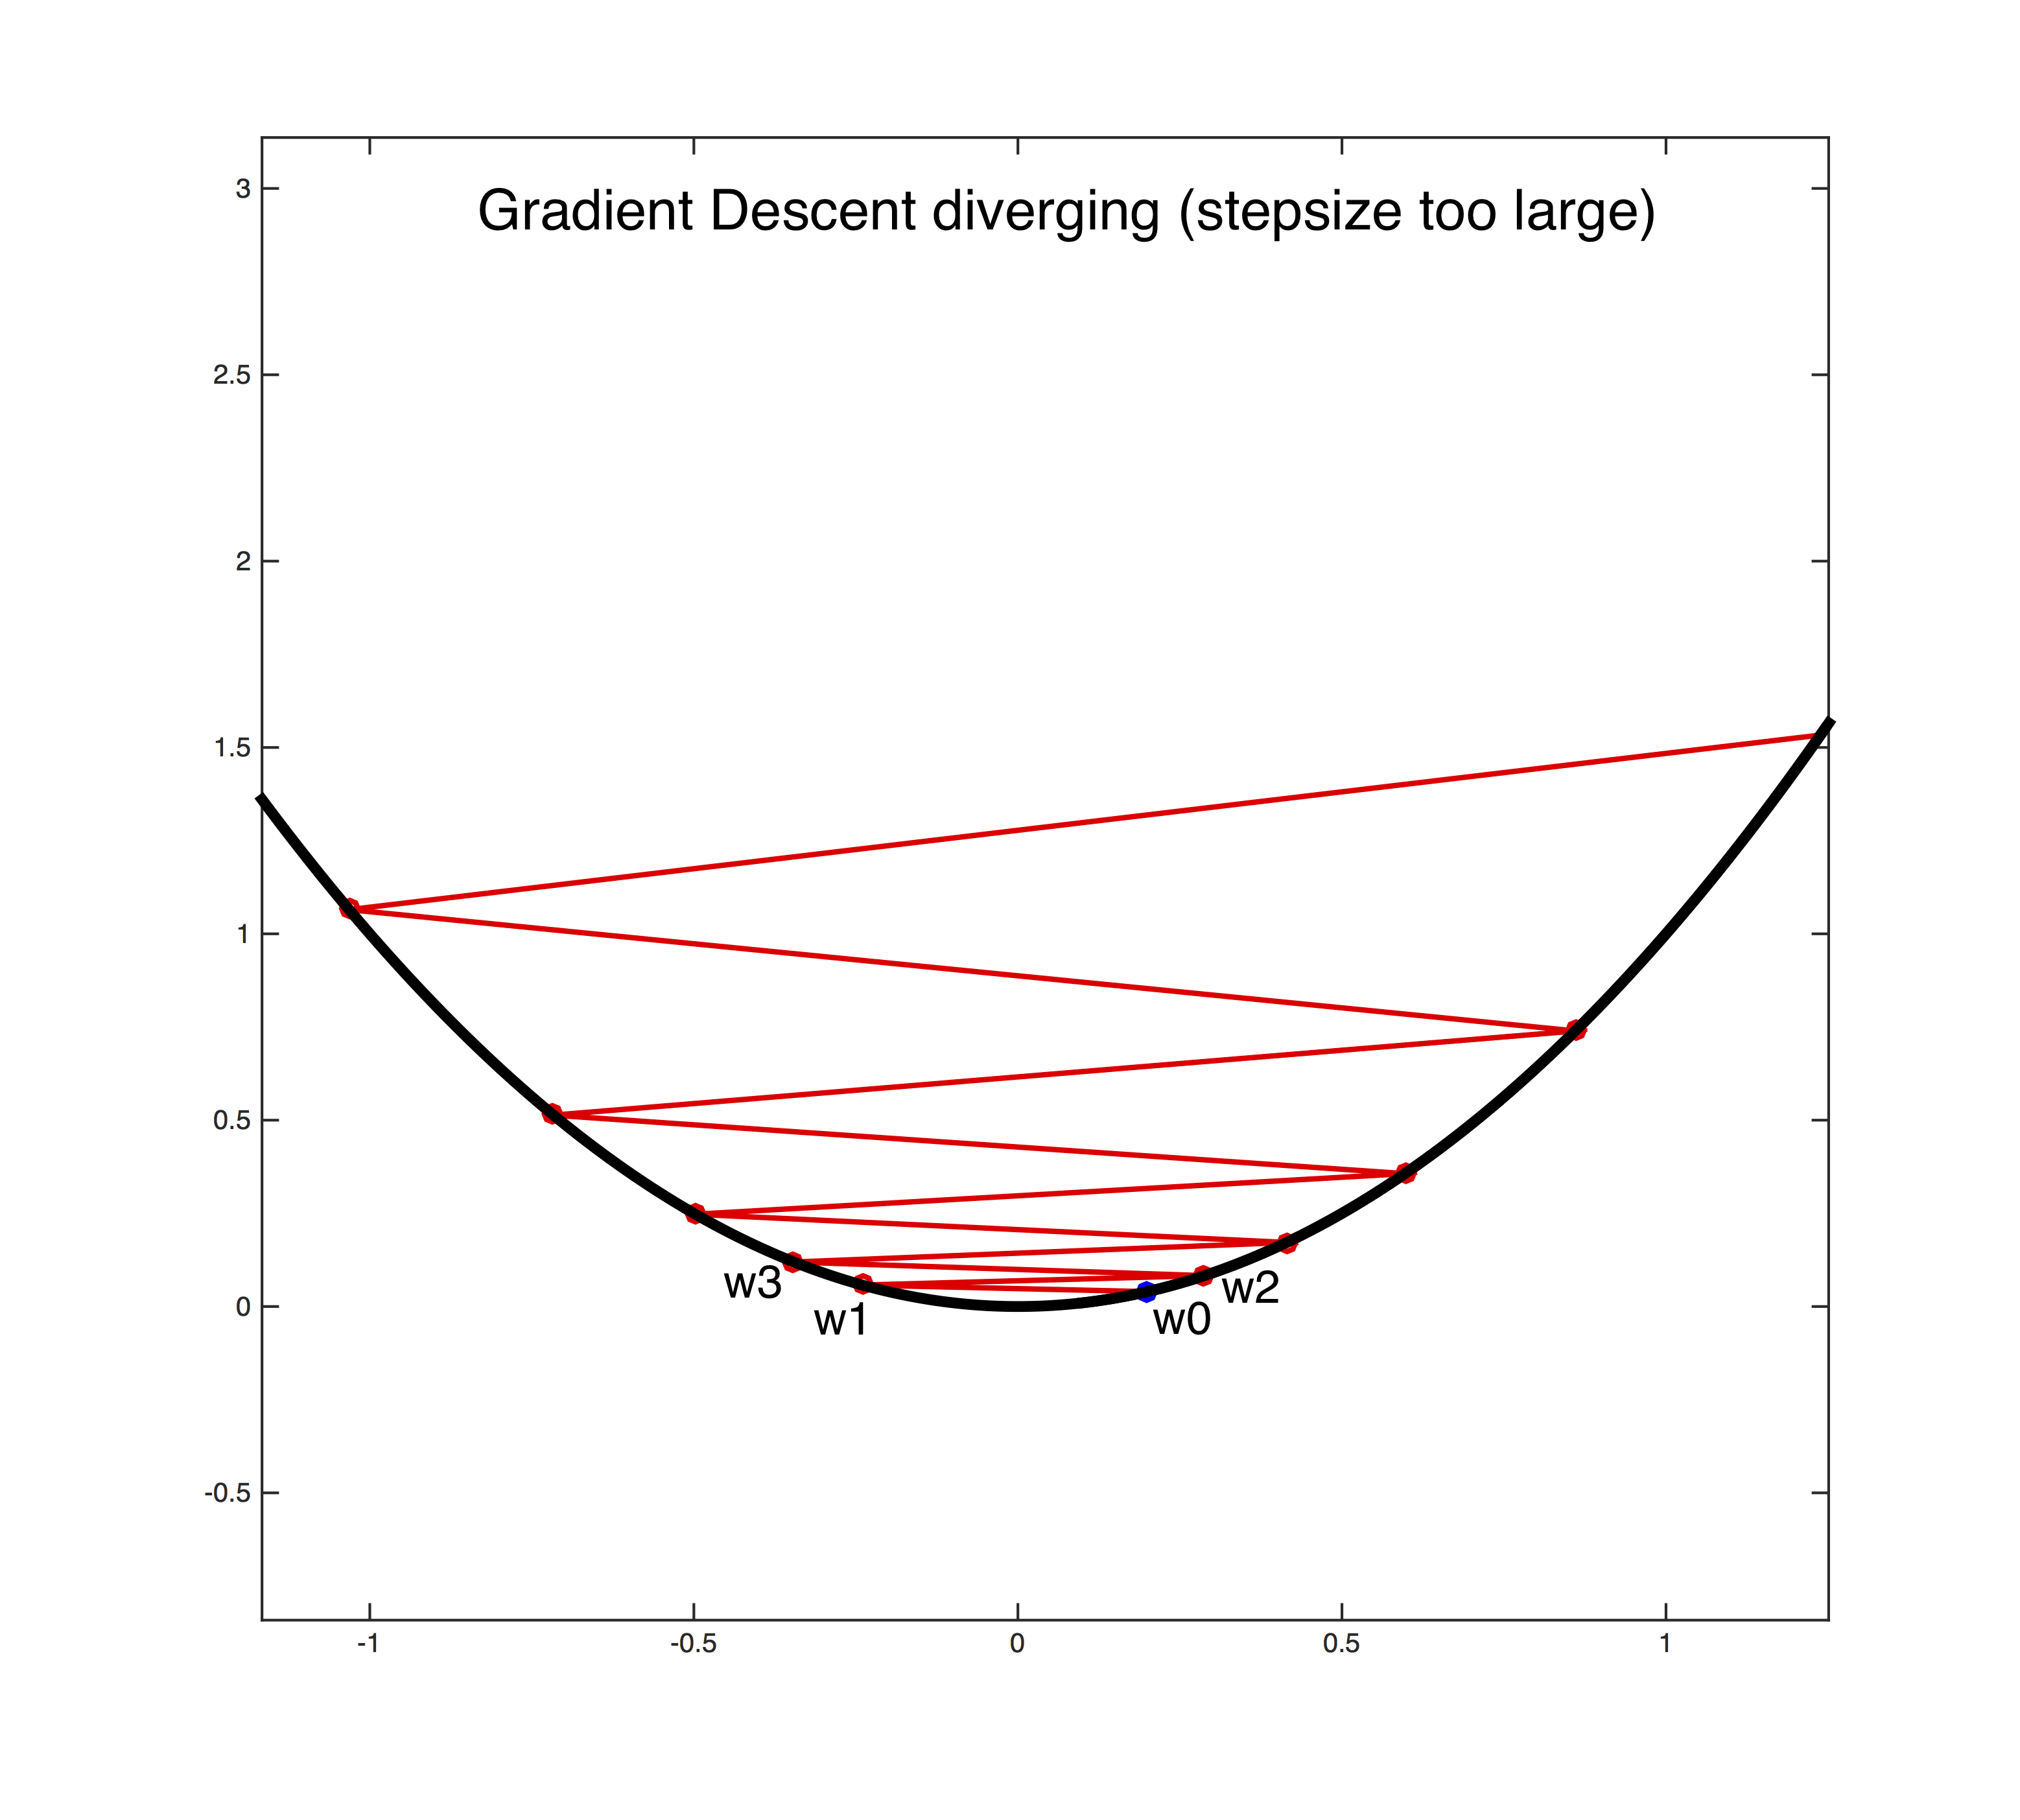
\includegraphics[width=7cm]{./Figs/lr_diverge.jpg} }}%
    \caption{Consequence of choosing $\alpha$ \cite{Cornell}}%
    \label{fig:learningrate_example}%
\end{figure}

\subsection{Batch, Mini Batch, and Stochastic Gradient Descent}

\begin{definition} [Epoch]
    An epoch is one complete pass of the training dataset
\end{definition}

\begin{definition}[Batch Gradient Descent]
    Also known simply as gradient descent, describes a method that updates the parameters ($W$ and $b$) using the \emph{whole training dataset per epoch}. For example, one would use the mean of the gradients of all the training data to update the parameters. However it is wasteful to compute the loss function over the entire training set in order to perform a parameter update only once \cite{Stanford}.
\end{definition}

\begin{definition}[Stochastic Gradient Descent]
    Also known as on-line gradient descent, describes a method that updates the parameters after every \emph{single} training data. When people refer to SGD, they usually refer to minibatch gradient descent approach as it is more commonly used. The stochastic gradient descent is technically a minbatch gradient descent with a batch size of 1. 
\end{definition}

\begin{definition}[Minibatch Gradient Descent]
    Is a method that updates the parameters on every subset with a batch size, $B$, of the training dataset per epoch. The batch size is a hyperparameter which are chosen because of memory constraints. The batch size is usually in powers of 2 because vectorized operations work faster when the inputs is the power of 2 \cite{Stanford}. 
\end{definition}

\begin{thebibliography}{2}
    \bibitem{DrCoop} Cooper.

    \bibitem{UoT} Mengye Ren and Matthew MacKay, UoT CSC 411, Winter 2019. \url{https://web.archive.org/web/20190513201539/https://www.cs.toronto.edu/~mren/teach/csc411_19s/lec/lec06.pdf}

    \bibitem{Cornell} Kilian Q. Weinberger, Cornell CS4780, Fall 2018.
    \url{https://web.archive.org/web/20180827054501/https://www.cs.cornell.edu/courses/cs4780/2018fa/lectures/lecturenote01_MLsetup.html}
     \url{https://web.archive.org/web/20181016051558/https://www.cs.cornell.edu/courses/cs4780/2018fa/lectures/lecturenote07.html}

    \bibitem{Stanford} Fei-Fei Li, Jiajun Wu, and Ruohan Gao, Stanford CS231n, Spring 2022. \url{https://web.archive.org/web/20230109135558/https://cs231n.github.io/optimization-1/}

\end{thebibliography}

\end{document}
